\chapter[\paperItitle]{\texorpdfstring{%
		Using TPM Secure Storage in\\Trusted High Availability Systems}{%
		\paperItitle}}
\label{ch:tpmhas}
\paperRemark{\paperIref}

{
%\documentclass{llncs}
%\usepackage{multirow}
%\usepackage{rotating}
%\usepackage{tikz}
%\usetikzlibrary{arrows,backgrounds,positioning}
%\usepackage{enumitem}
%\usepackage{hyperref}
%\hypersetup{pdfborder=0 0 0}
%\usepackage{listings}
%\usepackage{booktabs}
%\usepackage{array}
%\usepackage{amsmath}
%\usepackage{amssymb}
%\newcolumntype{P}[1]{>{\centering\let\newline\\\arraybackslash\hspace{0pt}}m{#1}}
%\usepackage{geometry}

\makeatletter
\def\namedlabel#1#2{\begingroup
    #2%
    \def\@currentlabel{#2}%
    \phantomsection\label{#1}\endgroup    
}
\makeatother

\newenvironment{tpmcommands}{\begin{scriptsize}}{\end{scriptsize}}

\section*{Abstract}

We consider the problem of providing trusted computing functionality in high availability systems. We consider the case where data is required to be encrypted with a TPM protected key. For redundancy, and to facilitate high availability, the same TPM key is stored in multiple computational units, each one ready to take over if the main unit breaks down. This requires the TPM key to be migratable. We show how such systems can be realized using the secure storage of the TPM. Hundreds of millions TPM 1.2 chips have been shipped but with the recent introduction of TPM 2.0, more manufacturers are expected to start shipping this newer TPM. Thus, a migration from TPM 1.2 to TPM 2.0 will likely be seen in the next few years. To address this issue, we also provide an API that allows a smooth upgrade from TPM 1.2 to TPM 2.0 without having to redesign the communication protocol involving the different entities. The API has been implemented for both TPM 1.2 and TPM 2.0. 

\section{Introduction}
A High Availability System, hereafter referred to as HAS, can be used for mission critical systems like medical, trading, banking, mobile network infrastructure, and blue-light systems. Such systems often run for many years and sometimes longer than a decade.  As part of high availability requirements, often such systems need trusted platform functions that guarantee that only authentic and approved system software and applications can run on them. Also, one frequently sees demands to safely store sensitive data and keys used by applications and management functions.
%HAS and more TPMs
In the types of HAS that we consider there are multiple Computational Units (CUs) that are organized so they can take over each others' tasks in the event a CU fails. To provide for trusted platform functions like authenticated boot and storage of sensitive data and keys, each CU is equipped with a TCG Trusted Platform Module (TPM). Typically, a CU is a PCB or rack mountable unit that can be inserted in a cabinet that hosts the HAS, and can accommodate a multitude of CUs. The use of multiple TPMs for protection in a HAS has many technical problems due to the migration problems that the use of TPM introduces.
 
At the same time, there are different versions of the TPM, which in some aspects are very different from each other. TPM 1.2 was introduced in 2003 and since 2006 a TPM chip has been included in many laptops. In 2012, TPM 2.0 was introduced, adding new functionality and with no backwards compatibility with TPM 1.2. Even though PCBs still come equipped with a TPM 1.2 chip, within a few years TPM 2.0 is likely to be the dominant chip on newer boards. This provides a challenge as systems utilizing trusted computing functionality may have to undergo significant, and costly, changes.
 
In this paper, we focus on Trusted Computing Technology, and how a CU manufacturer can offer a solution where customers have unique keys, only usable in a specific HAS, but which still utilizes generic CUs to be used as replacement boards. Moreover, we provide a general API that is independent of the TPM version used. This allows for a cost-efficient deployment of the system as it can be easily updated when TPM 2.0 gains widespread adoption.

The paper is organized as follows. Section~\ref{sec:overview} gives a brief overview of TPMs, describing some functionality relevant to the paper. In Section~\ref{sec:usecase}, we specify the use cases together with the threat model. In Section~\ref{sec:requirements} we describe the requirements that must be met by the proposed solution, which is then described in Section~\ref{sec:sol}. A security analysis of the proposed solution is described in Section~\ref{sec:secanalysis}. Section~\ref{sec:unifiedapi} describes the general API. Finally we discuss some related work in Section~\ref{sec:tpmhas:relatedwork}. Section~\ref{sec:conc} concludes the paper.
 
\section{Overview of TPM 1.2 and TPM 2.0}
\label{sec:overview}
TPMs have been around for more than a decade and most laptops ship with a TPM. Still, we have seen very few applications taking advantage of the functionality provided by TPMs. Microsoft's Bitlocker encryption system is the most known and widely used. A TPM enables trusted computing functionality such as authenticated boot, remote attestation and sealed storage. This section will give a short introduction to TPM 1.2 and 2.0, highlighting the differences when duplicating keys to new destinations. For a more detailed treatment we refer to the specifications~\cite{TPM1.2spec,TPM2.0r07}.
 
\subsection{Overview of TPM 1.2 and Certifiable Migration Keys}
A TPM 1.2 provides a key hierarchy of asymmetric keys, where the private part of a child key is protected (encrypted) using the public key of the parent. Parents are of type \textit{storage key} and are used to encrypt other keys, while leafs in the tree can be of any type, e.g., a signing key, encryption key or attestation identity key (AIK). Asymmetric keys in TPM 1.2 consist of two parts: one public part, and one private part. The public part contains data such as the public key and different flags. The private part is encrypted, and contains the private key, but also usage and migration secrets. The root of the key hierarchy is the Storage Root Key (SRK), which is created when someone takes ownership of the TPM. The TPM owner authenticates using an \textit{owner secret} and several commands require owner authorization, e.g., commands used in migration which is the main topic of this paper. Commands that use the private part of a key are authenticated using a \textit{usage secret} which can be unique to each key. Such commands are e.g., creation of new keys, data signing and data decryption.
 
The only way to have the same key protected by two TPMs is to use migratable keys. Migratable keys were introduced in TPM 1.1, offering the ability to migrate (or actually duplicate) a TPM protected key to another TPM. There are two variants of migration schemes specified, called \textit{rewrap} and \textit{migrate}. In the rewrap case, the private part of the migratable key is simply decrypted and re-encrypted using the destination key. In the migrate scheme, the key is instead re-encrypted using the public key of a migration authority (MA). The MA can then re-encrypt the private part with the destination public key. We will not consider the scheme using a migration authority any further in this paper.

Each key also has a \textit{migration secret} in addition to the usage secret. Migration is only allowed if the migration secret is known. For non-migratable keys, the migration secret is \textit{tpmproof}, a value internal to the TPM and never exposed. Also, the source TPM-owner must approve the destination, however, for any migratable key, the owner can choose any destination. Thus, if the TPM owner is not trusted, the key can end up in any TPM, or even outside a TPM if the owner migrates the key to his own keypair generated by e.g., OpenSSL.

A Certifiable Migration Key (CMK), introduced in TPM 1.2, allows for a trusted entity, called Migration Selection Authority (MSA), to be in control of destinations for each individual CMK. The MSA control is tied to each CMK by binding the CMK key to a list of MSAs at key creation time (called \textit{MSAList}). Similar to migratable keys, there are two possible migration schemes for CMKs, \textit{restrict\_migrate} and \textit{restrict\_approve}. In restrict\_approve, tickets which include both the CMK and the destination public key, are used to control the destination. Tickets are signed by the MSA and only the destination in the ticket can be used as target for migration. Then the ticket is first used to create a CMK blob encrypted with the destination SRK. Then the ticket is used again in the target TPM to convert the blob into a key in the key hierarchy. The tickets signed by the MSA are called restrictTickets. From these tickets, sigTickets are produced by letting the TPM owner approve the information in the restrictTicket. Thus, both the MSA and the TPM owner control the migration of a CMK. In the following, restrictTickets will sometimes simply be denoted ``ticket'' since this is the ticket that will be communicated between entities.

In the restrict\_migrate scheme, the CMK is migrated directly to an MSA. No ticket is needed in this case since the key already is bound to the MSA at creation time so the MSA is trusted as destination.
 
Different from a migratable key, a CMK can be certified by an AIK. The certification states that the CMK key belongs to a TPM and that the private part of the key will never leave the TPM in unencrypted form (assuming the MSA enforces this). Certification of CMKs is not used in this paper and will not be considered further.
 
 
\subsection{Limitations of CMKs}
The TPM owner controls migratable keys in the sense that he/she can create them outside of the TPM or migrate them out from the TPM. Thus, there is no guarantee that the private key is TPM protected. While this problem is addressed by CMKs, putting an MSA in control, the CMKs have some important limitations.
\begin{itemize}
\item A software MSA can create CMK keys outside the TPM and migrate them into a TPM.
\item When the restrict\_migrate scheme is used, a software MSA can read the private CMK key.
\item Each time a CMK is migrated, both out of a TPM and into a new TPM, a signed ticket from an MSA is required. Thus, from the perspective of the two TPMs, there must be communication with a third party. If tickets are created in advance this is not required, but then the destinations must be known in advance.
\end{itemize}
 
The last limitation above significantly restricts the use of CMKs in HAS's, because the destination CU (e.g. a replacement unit) is not known in advance. It is therefore important to find secure ways to combat this problem. This is one of the main goals in our proposed design.
 
\subsection{Overview of TPM 2.0 and Duplication}
The key hierarchy in TPM 1.2 has been replaced by an object hierarchy in TPM 2.0. Objects in the hierarchy can be both symmetric and asymmetric keys, but also data blobs. The type is determined by a combination of the binary properties \textit{sign}, \textit{decrypt} and \textit{restricted}, where the last property means that the object (key) can only perform actions on data prepared by the TPM itself. This is controlled by including a specific byte sequence in these objects. Some commands can only be performed in objects with this byte sequence. Storage keys are asymmetric keys with the properties restricted and decrypt. Similar to TPM 1.2, these keys protect child keys in the hierarchy. However, the protection in TPM 2.0 is by symmetric encryption. A storage key has a unique seed in its private part, which is used to derive a symmetric encryption/decryption key. This key is derived from the seed each time a new object is created or loaded into the TPM.
 
In TPM 2.0 the term migration has been replaced by duplication, as it more accurately reflects the reality.
%A duplicated key, or migrated in TPM 1.2, is not removed from the source TPM.
Two important object attributes are used to control duplication of a key. The first, fixedTPM, controls if an object can be duplicated at all. If an object has this attribute set, the object can not be duplicated. Naturally, an object with fixedTPM set can not be below an object with fixedTPM clear in the hierarchy. The second, fixedParent, controls if an object can be explicitly duplicated (when fixedParent is clear) or if it must be implicitly duplicated (when fixedParent is set) by duplicating a parent key, which has fixedParent clear.
 
The notion of CMKs and migration schemes has been completely removed in TPM 2.0, and has been replaced by \textit{policies}. A policy is a general concept that controls the actions that can be performed on an object in the hierarchy. Policies are set upon object creation time by storing a value, called authPolicy, in the public part of an object. The authPolicy is a hash value created by running several policy commands, where each command extends the authPolicy digest. This is similar to how PCR values are built by using TPM\_Extend. The authPolicy can be based on e.g., time limitations on usage of the object, specific commands that are possible to execute with an object and specific parameters that can be used in a command. Before executing a command a policyDigest must be built in a policy session. This session also stores specific context values that are checked upon execution, e.g., the command code if a certain command must be executed or the fact that a certain authorization method should be used. The final policyDigest is compared to the object's authPolicy and if they match, the command is executed using the information in the context values. Policies can be combined using logical AND and OR.
 
The use of policies is in general optional as it is possible to authorize using HMAC, similar to authorization in TPM 1.2, or by directly providing a password. However, for duplication the use of policies is mandatory. Policy commands that are particularly interesting for key duplication are TPM2\_PolicyAuthorize and TPM2\_PolicyDuplicationSelect.
 
The TPM2\_PolicyAuthorize command allows a policy to change by letting an authority sign the new policy. This is done as follows. The TPM user generates a new policy to use for an object. This policy, and the properties it represents, are evaluated by an authority. If they are acceptable, the authority signs this policy and returns the signature. The signature is verified using TPM2\_VerifySignature which returns a ticket showing that the signature is valid. This ticket, together with the approved policy, is then used in the TPM2\_PolicyAuthorize command. Upon executing this command with a valid ticket, the policyDigest is updated by replacing it by the hash of the name of the signature key. This hash is then the new PolicyDigest. Thus, any policy that needs to change during the lifetime of an object needs to include the TPM2\_PolicyAuthorize command after all policies that are subject to change. Policies added after this command has been executed can not be changed.
 
The TPM2\_PolicyDuplicationSelect command is used to control the destination for a duplication. The command includes both the name of the object to be duplicated and the name of the destination. The policyDigest is updated using both these names. Thus, the policy ties the object to a specific destination (or several if logic OR is used). Since the destination is typically not known when an object is created, this is typically used together with TPM2\_PolicyAuthorize. This will allow an authority to verify that the destination is valid and then sign the resulting policyDigest.

\subsection{Platform Configuration Registers}
All TPMs, both of version 1.2 and 2.0, have a number of Platform Configuration Registers (PCRs). These registers store a hash value, which is built-up by repeatedly calling TPM\_Extend or TPM2\_Extend. This creates a cumulative hash, since an extend operation depends on both a new value and the previous PCR value. The PCRs are used to store measurements of the hardware configuration and software. The measured values are stored in the Stored Measurement Log (SML), outside the TPM, while the digest are secured by the TPM.

The SML can be read to ensure that the measurement values of the system are as expected, and the integrity of the SML can be verified by comparing them to the PCRs. In addition, keys in the TPM can be bound to certain PCR values, such that keys can only be used when the PCRs have the correct value, thus ensuring that keys are only used in a trusted hardware and software setting.

\section{Scenario and Threat Model}
\label{sec:usecase}
The considered use case aims at building a robust infrastructure, taking the HAS life cycle into consideration. The scenarios includes four entities.

The hardware, i.e., the computational units (CUs), are produced by a \textbf{CU manufacturer}. The CU boards will include a TPM but it will not be associated with any particular, or identified, customer or end user.

A HAS is assembled by a \textbf{HAS manufacturer}. The HAS manufacturer takes two or more CUs, due to the redundancy requirements, from the CU manufacturer and assembles the HAS, also using equipment from other sources. This additional equipment is outside the scope of this work.

\textbf{Customers} are purchasing a HAS on which they want to store sensitive data. This data can e.g., be keys or sensitive application data of applications running on the HAS. The sensitive data is stored in \textit{secure storage}, meaning that it resides on a hard disk in encrypted form, protected by a TPM. 

A \textbf{Trusted Third Party} (TTP) is used to enable the secure migration of keys between TPMs. This is the MSA in TPM 1.2 and authority in TPM 2.0. We assume that this party keeps all keys secure, possibly, but not necessarily, with a TPM. %A TTP is also used to guarantee that attestation identity keys in TPM 1.2 belong to a TPM. This is called PrivacyCA in TCG. The two TTPs are typically different entities and when we refer to TTP in this paper we mean the MSA/Authority. 

\subsection{Threat Model}
Any attacker that controls the hardware, will also be able to circumvent the protection offered by trusted computing, as the root of trust is potentially compromised. Thus, to this end it is natural to consider the CU manufacturer trusted and it can theoretically be merged with the TTP. It is also from the CU manufacturer's perspective we mainly treat the problem. Still, mounting an attack against the hardware is different from attacking the software controlling the migration on the TTP. We will therefore consider them as separate entities. % in this paper.
%TODO: Still, some attacks are easier to mount than others and a separation can be motivated if.....\textit{how to deal with this, should we merge them?? What is included in our threat model}

In practice, many service and operating personnel, hereafter collectively named company employees, will have access to the HAS during its lifetime. Not all company employees can be considered trusted, and this is the main reason to protect data using a TPM, as the decryption key will never leave the TPM unencrypted. Not trusting company employees will also help the customer to protect against other, potentially malicious, customers' personnel.

\begin{itemize}
\item[\namedlabel{TcustEmployees}{T1}.] Anyone, including customer employees, can copy data and software from drives in the HAS cabinet. They may also interact with the TPM.
\item[\namedlabel{Tstolen}{T2}.] CU boards can be stolen, both spare boards and those already mounted in a cabinet. Boards from customer A can be used in the HAS of customer B.
\item[\namedlabel{THAS}{T3}.] HAS manufacturer employees can access data in the HAS when it is being assembled, in particular data that is associated with the TPM.
\end{itemize}

The main goal is to protect stolen (encrypted) HAS data from being accessed in cleartext, while at the same time provide a system with very low downtime. 

\section{Requirements} \label{sec:requirements}
Based on the scenario and threat model, we define the following requirements.

\begin{itemize}
\item[\namedlabel{Rsecurity}{R1}.] \textbf{Data confidentiality.} Data stored on secondary memory, e.g., hard drives or memory cards, must always be encrypted. The key may never be stored (unencrypted) on secondary memory.
\item[\namedlabel{Rredund}{R2}.] \textbf{Redundancy.} The data on a HAS must at all times be accessible, even in the case of hardware failure.
\item[\namedlabel{Rscale}{R3}.] \textbf{Scalability.} After completed assembly by the HAS manufacturer, spare CUs can be ordered by the customer directly from the CU manufacturer. These are generic and not personalised for the specific customer. Thus, we assume that anyone will be able to buy a generic CU.
\item[\namedlabel{RcustLock}{R4}.] \textbf{Customer lockdown.} Only TPMs initiated by the CU factory can be used as replacement boards. This will allow the CU factory to create boards that are specific for a group of customers, still allowing customers to have unique keys.
\item[\namedlabel{Rpers}{R5}.] \textbf{TPM Compatibility.} The API used by the different entities must be compatible with both TPM 1.2 and TPM 2.0.
\item[\namedlabel{RcustControl}{R6}.] \textbf{Customer control.} The customer should be the owner of the TPM, allowing him to use it for other purposes such as remote attestation and key certification. This also allows the customer to reuse the hardware and TPMs in the event of a CU manufacturer going out of business.
\item[\namedlabel{RuserF}{R7}.] \textbf{User friendliness.} Replacing CUs in the HAS should be as easy as possible for the customer. This includes minimizing the online communication with other entities, possibly providing a completely offline solution. It also includes minimizing the HAS interaction needed by customer employees.
\end{itemize}

We return to these requirements in Section~\ref{sec:secanalysis} when evaluating the security of the proposed solution.


For the sake of simplifying our expositions we assume further that the HAS uses only two CUs. Thus, the key protecting the sensitive data must be identical in both TPMs so that the backup CU can immediately become active in case the first CU fails. Further, when a CU breaks it should be replaced by a spare CU from the CU manufacturer.

\section{Proposed System Design}
\label{sec:sol}
Due to the redundancy requirement (\ref{Rredund}), one key must be associated with several TPMs. This can only be done using duplicable (migratable in TPM 1.2) keys. We first analyze how this can be achieved in TPM 1.2. Consider the most straightforward solution of having a plain migratable key immediately below the SRK in the hierarchy. To migrate this key to a new SRK, the TPM owner can simply rewrap this key with the new SRK and import it to the new TPM.

\begin{scriptsize}
\begin{verbatim}
TPM_AuthorizeMigrationKey     //Owner authorized
TPM_CreateMigrationBlob       //On source TPM
TPM_ConvertMigrationBlob      //On destination TPM
\end{verbatim}
\end{scriptsize}
The main problem with this is that the owner can rewrap the key with any key, even one created outside the TPM. Thus, if the customer is the owner (\ref{RcustControl}) the private part of the key is not guaranteed to be protected by the TPM at all times (\ref{TcustEmployees}).

With CMK keys in TPM 1.2 and policies in TPM 2.0, the migration/duplication can be controlled by a trusted authority, even when the customer is the TPM owner. The migration of a key then proceeds as follows.

\begin{scriptsize}
\begin{verbatim}
TPM_CMK_ApproveMA              //On source TPM, owner authorized
TPM_CMK_CreateKey              //On source TPM
TPM_AuthorizeMigrationKey      //On source TPM, owner authorized
TPM_CMK_CreateTicket           //On source TPM, owner authorized
TPM_CMK_CreateBlob             //On source TPM
TPM_CMK_CreateTicket           //On destination TPM, owner authorized
TPM_CMK_ConvertMigration       //On destination TPM
\end{verbatim}
\end{scriptsize}
The \verb!TPM_CMK_ApproveMA! command lets the owner bind an MSA to the CMK. The ticket is signed by the MSA and the key can only be migrated to a destination given in the ticket. From this it is clear that the customer can not be owner at the time the key is first created since he could assign any key to be an MSA public key.

An important observation is that a TPM key, we call it $K_{e}$ ($e$ for encryption), can be used on several TPMs provided that the parent key $K_p$ is the same on all TPMs. The key blob is stored on (secondary) memory and loaded into the TPM when needed. Upon loading a key, it is decrypted by the parent key. Thus, if the parent key is $K_p$ it can be loaded into any TPM that has $K_p$ in the key hierarchy. In order to have $K_p$ in several TPM key hierarchies, it must be migratable and any key having a migratable key as parent key must also be migratable. Moreover, a CMK (which is migratable) may not have a migratable key as parent. Figure~\ref{migratableHierarchy} summarizes these restrictions.

\begin{figure}[h]
\centering
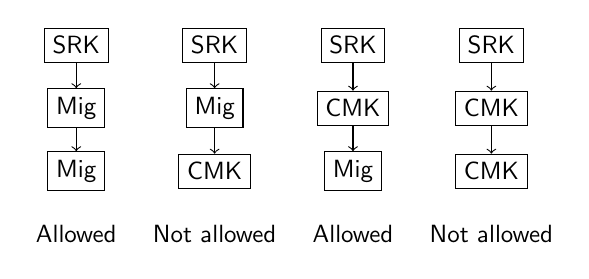
\begin{tikzpicture}[font=\sffamily]
%Case A
\begin{scope}[xshift=0]
\node[draw,align=center, scale = 0.9] (SRK) at (0,0) {SRK};
\node[draw,align=center, scale = 0.9] (mig1) at (0,-0.8) {Mig};
\node[draw,align=center, scale = 0.9] (mig2) at (0,-1.6) {Mig};
\node[align=center, scale = 0.9] (CaseA) at (0,-2.4) {Allowed};
\draw[->] (SRK.south) -- (mig1.north);
\draw[->] (mig1.south) -- (mig2.north);
\end{scope}
%Case B
\begin{scope}[xshift=50]
\node[draw,align=center, scale = 0.9] (SRK) at (0,0) {SRK};
\node[draw,align=center, scale = 0.9] (mig) at (0,-0.8) {Mig};
\node[draw,align=center, scale = 0.9] (cmk) at (0,-1.6) {CMK};
\node[align=center, scale = 0.9] (CaseA) at (0,-2.4) {Not allowed};
\draw[->] (SRK.south) -- (mig.north);
\draw[->] (mig.south) -- (cmk.north);
\end{scope}

%Case C
\begin{scope}[xshift=100]
\node[draw,align=center, scale = 0.9] (SRK) at (0,0) {SRK};
\node[draw,align=center, scale = 0.9] (cmk) at (0,-0.8) {CMK};
\node[draw,align=center, scale = 0.9] (mig) at (0,-1.6) {Mig};
\node[align=center, scale = 0.9] (CaseA) at (0,-2.4) {Allowed};
\draw[->] (SRK.south) -- (cmk.north);
\draw[->] (cmk.south) -- (mig.north);
\end{scope}

%Case D
\begin{scope}[xshift=150]
\node[draw,align=center, scale = 0.9] (SRK) at (0,0) {SRK};
\node[draw,align=center, scale = 0.9] (cmk1) at (0,-0.8) {CMK};
\node[draw,align=center, scale = 0.9] (cmk2) at (0,-1.6) {CMK};
\node[align=center, scale = 0.9] (CaseA) at (0,-2.4) {Not allowed};
\draw[->] (SRK.south) -- (cmk1.north);
\draw[->] (cmk1.south) -- (cmk2.north);
\end{scope}


\end{tikzpicture}
\caption{Key hierarchy restrictions for migratable keys. Both the \texttt{TPM\_CMK\_CreateKey} and the \texttt{TPM\_CMK\_ConvertMigration} commands verify that the parent key is not migratable.}
\label{migratableHierarchy}
\end{figure}

Thus, if we wish to be able to use $K_{e}$ in several TPMs without having to migrate it, this key must be migratable, but not a CMK. The parent key $K_p$ can be either a plain migratable key or a CMK. Since $K_p$ must be explicitly migrated between TPM to facilitate the use of $K_{e}$, we make use of a trusted third party that can control this migration. On a very high level, the proposed solution is given in Fig.~\ref{fig:overviewDesign} and can be summarized as follows.

\begin{figure}[hbtp]
	\centering
	\resizebox{100mm}{!}{
	\begin{tikzpicture}[node distance=1.9cm,auto,>=latex',scale=1, every node/.style={scale=1}, font=\sffamily]
		%\def\ts{\footnotesize}
		% Kp things
		\def\ts{\small}
		\node (cu) at (0,0) {\textbf{CU factory}};
		\node[right=of cu] (authority) {\textbf{TTP}};
		\node[right=of authority] (has) {\textbf{HAS factory}};
		\node[right=of has] (customer) {\textbf{Customer}};

		\node[below=0.5cm of authority] (genkey) {\ref{item:genkp}: generate $K_p$};
		\draw[->] ([yshift=-2cm]cu.center) -- node [midway] {\ts \ref{item:sendsrk}: SRK, cert(SRK)} ([yshift=-2cm]authority.center);
		\node[below=2.2cm of authority] (genkey) {\ref{item:migratetocusrk}: place $K_p$ under SRK};		
				
		\draw[<-] ([yshift=-3.5cm]cu.center) -- node [midway] {\ts \ref{item:sendkp}: $K_p$} ([yshift=-3.5cm]authority.center);

		\node (loadblob) at ([xshift=0.5cm,yshift=-4.0cm]cu.south) {\ref{item:culoadblob}: load $K_p$};

		\draw[->] ([yshift=-5.0cm]cu.center) -- node [midway] {\ts CU} ([yshift=-5.0cm]has.center);
		\node (initialization) at ([xshift=-0.5cm, yshift=-0.2cm]cu.south) [draw,dashed,minimum width=8cm,minimum height=5.0cm,anchor=north west] {};
		
		% Generate Ke things
		\node (kegeneration) at ([xshift=-0.7cm, yshift=-0.2cm]initialization.south) [draw,dashed,minimum width=8.2cm,minimum height=1.2cm,anchor=north west] {generate $K_e$};
		
		% Send new CU things
		\node (sendnewcu) at ([xshift=-7.43cm, yshift=-0.2cm]kegeneration.south) [draw,dashed,minimum width=11.5cm,minimum height=1.2cm,anchor=north west] {};
		\draw[->] ([yshift=-0.1cm, xshift=0.4cm]sendnewcu.west) -- node [midway] {\ts Send replacement CU} ([yshift=-0.1cm, xshift=-0.4cm]sendnewcu.east);
	\end{tikzpicture}
	}
	\caption{Overview of the proposed system}
	\label{fig:overviewDesign}
\end{figure}


\begin{enumerate}
\item The TTP generates the CMK key $K_{p}$ to be included in all new TPMs.  \label{item:genkp}
\item The CU manufacturer takes ownership of a new TPM and asks the TTP for $K_p$ to be migrated under the new SRK. \label{item:sendsrk}
\item The TTP migrates the key to the given SRK. \label{item:migratetocusrk}
\item The TTP sends migrated key, encrypted with the SRK public key, to the CU factory. \label{item:sendkp}
\item The CU factory loads the key into the CU. \label{item:culoadblob}
\end{enumerate}

At this point, a generic board has been prepared with a unique SRK, and the $K_p$ which is common for all boards created by the same CU.
The boards are now prepared to be shipped either to a HAS factory for HAS assembly, or to a customer as replacement for a broken board. Assume it has been sent to a HAS factory. The next step is then to generate the customer specific key $K_e$. We consider three different alternatives for generating $K_e$, namely a TTP generated $K_e$, a HAS generated $K_e$, and a customer generated $K_e$. 

Since the boards are generic, we must take two important aspects into account. First, since $K_e$ is a migratable key in TPM 1.2, we must ensure that it can not be migrated further by a malicious customer employee (knowing the owner secret). This can be controlled by not disclosing the migration secret to untrusted users, i.e., simply to destroy it after key generation. In TPM 2.0 this can be controlled more easily by using the fixedParent attribute. Second, we must also ensure that $K_e$ is bound to the HAS, so it can not be used by other customers. This can be done by restricting the use of the key to a given PCR setting. In TPM 1.2, the PCR settings can be directly specified in the key structure, while in TPM 2.0 this is achieved using policies.

\subsection{TTP Generated $K_e$} \label{sec:ttpgeneratedke}
If the $K_e$ is generated by the TTP, the customer needs to send the PCR values which the new key should be bound to. Note that this requires online communication between the two entities. The new key will only be loadable under $K_p$, and only usable on a HAS with the correct PCR values. The steps can be described as in Figure~\ref{fig:ttpgeneratedke}.
\begin{figure}[hbtp]
	\centering
	\resizebox{80mm}{!}{
		\begin{tikzpicture}[node distance=1.9cm,auto,>=latex',scale=1, every node/.style={scale=1}]
		\def\ts{\small}
		\node at (0,0) (authority) {\textbf{TTP}};
		\node[right=of authority] (has) {\textbf{HAS factory}};
		\node[right=of has] (customer) {\textbf{Customer}};
		
		\node[below left=0.6cm and 0.0cm of customer,right] (readpcrs) {read PCRs};
		\draw[<-] ([yshift=-1.4cm]authority.center) -- node [midway] {\ts PCRs} ([yshift=-1.4cm]customer.center);
		\node[below=1.4cm of authority] (genkey) {create key};		
		
		\draw[->] ([yshift=-2.2cm]authority.center) -- node [midway] {\ts $K_e$} ([yshift=-2.2cm]customer.center);
		
		\node[right] (loadke) at ([yshift=-2.3cm]customer.south west) {load $K_e$};
		\end{tikzpicture}
	}
	\caption{TTP generated $K_e$}
	\label{fig:ttpgeneratedke}
\end{figure}

\subsection{HAS Manufacturer Generated $K_e$} \label{sec:hasgeneratedke}
If the HAS manufacturer generates $K_e$, it can be generated upon HAS assembly. The customer specific key is created on one CU, and then the blob is copied and loaded on the other CU as well. See Figure~\ref{fig:hasgeneratedke} for the executed steps.
\begin{figure}[hbtp]
	\centering
	\resizebox{80mm}{!}{
		\begin{tikzpicture}[node distance=1.9cm,auto,>=latex',scale=1, every node/.style={scale=1}]
		%\def\ts{\footnotesize}
		% Kp things
		\def\ts{\small}
		\node at (0,0) (authority) {\textbf{TTP}};
		\node[right=of authority] (has) {\textbf{HAS factory}};
		\node[right=of has] (customer) {\textbf{Customer}};
		
		\node[below left=0.5cm and 0.0cm of has,right] (readpcrs) {read PCRs};
		\node[below left=0.9cm and 0.0cm of has,right] (createkey) {create key};
		\node[below left=1.3cm and 0.0cm of has,right] (loadke) {load key};
		\end{tikzpicture}
	}
	\caption{HAS factory generated $K_e$}
	\label{fig:hasgeneratedke}
\end{figure}

\subsection{Customer Generated $K_e$} \label{sec:customergeneratedke}
The customer can execute the same steps as the HAS manufacturer in the section above to generate $K_e$. There is no difference in commands as the hardware is assembled in the same way as when it left the HAS manufacturer. Figure~\ref{fig:customergeneratedke} describes the commands.
\begin{figure}[hbtp]
	\centering
	\resizebox{80mm}{!}{
		\begin{tikzpicture}[node distance=1.9cm,auto,>=latex',scale=1, every node/.style={scale=1}]
		%\def\ts{\footnotesize}
		% Kp things
		\def\ts{\small}
		\node at (0,0) (authority) {\textbf{TTP}};
		\node[right=of authority] (has) {\textbf{HAS factory}};
		\node[right=of has] (customer) {\textbf{Customer}};
		
		\node[below left=0.5cm and 0.0cm of customer,right] (readpcrs) {read PCRs};
		\node[below left=0.9cm and 0.0cm of customer,right] (createkey) {create key};
		\node[below left=1.3cm and 0.0cm of customer,right] (loadke) {load key};
		\end{tikzpicture}
	}
	\caption{Customer generated $K_e$}
	\label{fig:customergeneratedke}
\end{figure}

\subsection{HAS Initialization}
Before leaving the HAS factory, and before creating the customer-specific keys, the HAS must personalize the HAS in such a way that the PCR values are unique to every customer. This ensures that customer-specific keys can be created.

When the HAS arrives to the customer, the customer must verify that the PCR values after system startup are indeed unique to the customer. This can be done by verifying that the Stored Measurements Log (SML) includes a hash that is customer dependent. If the HAS passes this test, it is ready to be used, knowing that $K_e$ can only be decrypted by this HAS. %For TTP and HAS generated $K_e$, this step is done after the creation of the key and for customer generated $K_e$ this is done prior to the generation of the key.

\section{\texorpdfstring{Security Analysis and Comparison of Properties for $K_e$ Generation}{Security Analysis and Comparison of Properties for Ke Generation}} \label{sec:secanalysis}
We assume that any data that resides on secondary storage on the HAS can be stolen by a malicious employee (\ref{TcustEmployees}). This includes the encrypted sensitive data, the encrypted sensitive part of a TPM protected key, and key usage secrets that are needed to use a key. While it could be possible to restrict the usage secret to only a small number of trusted employees, thus keeping it confidential, or to distribute it using secret sharing, we do not make such assumptions in this work. Since $K_e$ can only be used on a customer specific HAS, the encrypted sensitive part of $K_e$ can only be decrypted on this HAS. Thus, it is not possible to steal the encrypted data and the encrypted $K_e$ and decrypt the data using a generic board. The sensitive data is in clear only in primary memory, when used by the HAS software.

Since the boards are generic, a stolen board will not give an attacker any additional information compared to using their own boards. This mitigates threat~\ref{Tstolen}.

Threat \ref{THAS} can be mitigated to different extent depending on which $K_e$ generation alternative is used and which TPM version is used. When using a TTP for $K_e$ generation or when $K_e$ is generated by the customer, the HAS manufacturer employees will have no access to $K_e$ or any information about it. If $K_e$ is generated by the HAS manufacturer, for TPM 1.2, the security depends on the migration secret being destroyed after the key is generated. Otherwise, this key could be leaked to a malicious customer which is able to migrate $K_e$ outside the TPM. In TPM 2.0, $K_e$ is created with fixedParent set, which can be verified by the customer when the HAS is being initialized. Thus, it is only for HAS manufacturer created keys in TPM 1.2 that we are not able to fully mitigate \ref{THAS}, but it can be noted that an attack require cooperation between HAS manufacturer and customer employees. Returning to \ref{TcustEmployees}, we can also note that for customer created $K_e$ in TPM 1.2, we must ensure that the migration secret is destroyed. Thus, for TPM 1.2, higher security is achieved when $K_e$ is generated by a trusted third party. A summary of the different properties for different cases are given in Table~\ref{tbl:kesecanalysis}.

We note that there are three parts required to gain access to the secure information stored in the HAS: the encrypted data, the customer-specific key $K_e$, and the HAS itself. Thus, we cannot protect against cases where an attacker gets hold of all three of these parts. This includes a potential case where a malicious HAS employee cooperates with an malicious company employee at company A. If they have access to both stolen encrypted data, and the stolen $K_e$ from another company B, the HAS manufacturer and employee at A may cooperate to build a HAS with the same customer-specific PCR values as customer B, thus enabling them to decrypt the stolen data.

Finally, we also note that our analysis relies on the assumption that the TTP is trusted and available.

%\newcommand{\ayemark}{$\text{\rlap{$\checkmark$}}\square$}
\newcommand{\ayemark}{$\boxtimes$}
\newcommand{\nopemark}{$\square$}
%\newcommand{\ayemark}{OK}
%\newcommand{\nopemark}{X}

\begin{table}[hbtp]
	\begin{center}
		\caption{A summary of the properties when different entities generate the key $K_e$}
		\label{tbl:kesecanalysis}
		\begin{tabular}{m{3.65cm}l cc l cc l cc}
			\toprule
			& \phantom{w} & \multicolumn{2}{c}{TTP} & \phantom{w} & \multicolumn{2}{c}{HAS man.} & \phantom{w} & \multicolumn{2}{c}{Customer} \\
			\cmidrule{3-4} \cmidrule{6-7} \cmidrule{9-10}
			&& 1.2~~ & 2.0 & & 1.2 & 2.0 & & 1.2 & 2.0 \\
			\midrule
			{\small No online communication with other entity needed.}& & \nopemark & \nopemark && \ayemark & \ayemark && \ayemark & \ayemark \\
			\midrule
			{\small Possible to verify that $K_e$ is bound to $K_p$.}& & \ayemark & \ayemark && \nopemark & \ayemark && \nopemark & \ayemark \\
			\bottomrule
		\end{tabular}
	\end{center}
\end{table}

\section{Unified API} \label{sec:unifiedapi}

We have developed a unified API for the proposed functionality, such that a move from TPM 1.2 to TPM 2.0 will be as simple as possible.
By looking at the different phases of our solution, we can construct sequences of TPM commands for each of the two TPM versions, such that we get the same behaviour, abstracting away the differences between the TPM versions.

The API has been implemented and tested to ensure the correctness of the given commands, both for TPM 1.2 and TPM 2.0.
To do this, two different TPM simulators and support libraries have been used, one for each TPM version.

For TPM 1.2, IBM's Software TPM version 4720 \cite{ibmswtpm} has been used, which also includes \texttt{libtpm}, which can be used to interface with the simulator.
For TPM 2.0, Microsoft's TPM2 Simulator version 1.1 \cite{mstpm2sim} has been used, together with Microsoft's TPM Software Stack version 1.1 \cite{mstssmsr11}.

\subsection{Generation and Migration of $K_p$} \label{sec:unifiedapikp}

The first step in Figure~\ref{fig:overviewDesign} is to generate $K_p$. The following steps are executed on the TTP:
\begin{center}
	\begin{minipage}{0.4\linewidth}
		\begin{center}
			TPM 1.2
		\end{center}
		\begin{tpmcommands}
			\begin{verbatim}
			TPM_CMK_ApproveMA
			TPM_CMK_CreateKey
			\end{verbatim}
		\end{tpmcommands}
	\end{minipage}
	~~~~~~~~
	\begin{minipage}{0.4\linewidth}
		\begin{center}
			TPM 2.0
		\end{center}
		\begin{tpmcommands}
			\begin{verbatim}
			TPM2_PolicyAuthorize
			TPM2_Create
			\end{verbatim}
		\end{tpmcommands}
	\end{minipage}
\end{center}

In step~\ref{item:sendsrk}, the CU factory sends the SRK to the TTP, which then in step~\ref{item:migratetocusrk} executes the following commands to create a blob which is decryptable under the given CU's SRK.
\begin{center}
	\begin{minipage}{0.4\linewidth}
		\begin{center}
			TPM 1.2
		\end{center}
		\begin{tpmcommands}
			\begin{verbatim}
			TPM_AuthorizeMigrationKey
			TPM_CMK_CreateTicket
			TPM_CMK_CreateBlob
			\end{verbatim}
		\end{tpmcommands}
	\end{minipage}
	~~~~~~~~
	\begin{minipage}{0.4\linewidth}
		\begin{center}
			TPM 2.0
		\end{center}
		\begin{tpmcommands}
			\begin{verbatim}
			TPM2_LoadExternal
			TPM2_PolicyDuplicationSelect
			TPM2_PolicyAuthorize
			TPM2_Duplicate
			\end{verbatim}
		\end{tpmcommands}
	\end{minipage}
\end{center}

In step~\ref{item:sendkp}, the blob is sent to the CU factory, which then loads the blob into the TPM under the SRK (step~\ref{item:culoadblob}):
\begin{center}
	\begin{minipage}{0.4\linewidth}
		\begin{center}
			TPM 1.2
		\end{center}
		\begin{tpmcommands}
			\begin{verbatim}
			TPM_CMK_CreateTicket
			TPM_CMK_ConvertMigration
			TPM_LoadKey2
			\end{verbatim}
		\end{tpmcommands}
	\end{minipage}
	~~~~~~~~
	\begin{minipage}{0.4\linewidth}
		\begin{center}
			TPM 2.0
		\end{center}
		\begin{tpmcommands}
			\begin{verbatim}
			TPM2_Import
			TPM2_Load
			\end{verbatim}
		\end{tpmcommands}
	\end{minipage}
\end{center}

The CU now has $K_p$ loaded directly beneath the SRK, and the customer-specific key $K_e$ can be generated.

\subsection{Generation of $K_e$}
The customer-specific key $K_e$ can be generated using any of the alternatives given in Section~\ref{sec:ttpgeneratedke}, \ref{sec:hasgeneratedke}, and \ref{sec:customergeneratedke}.
The commands for each of the three cases are given below:

\subsubsection{TTP Generated $K_e$}
\begin{center}
	\begin{minipage}{0.4\linewidth}
		\begin{center}
			TPM 1.2
		\end{center}
		\begin{tpmcommands}
			\begin{verbatim}
			TPM_PcrRead       // customer
			// send PCRs TTP
			TPM_CreateWrapKey // TTP
			// send blob to customer
			TPM_LoadKey2      // customer CU1
			TPM_LoadKey2      // customer CU2
			\end{verbatim}
		\end{tpmcommands}
	\end{minipage}
	~~~~~~~~
	\begin{minipage}{0.4\linewidth}
		\begin{center}
			TPM 2.0
		\end{center}
		\begin{tpmcommands}
			\begin{verbatim}
			TPM2_PCR_Read  // customer
			// send PCRs to TTP
			TPM2_PolicyPCR // ttp
			TPM2_Create    // ttp
			// send blob to customer
			TPM2_Load      // customer CU1
			TPM2_Load      // customer CU2
			\end{verbatim}
		\end{tpmcommands}
	\end{minipage}
\end{center}


\subsubsection{HAS Manufacturer Generated $K_e$}
\begin{center}
	\begin{minipage}{0.4\linewidth}
		\begin{center}
			TPM 1.2
		\end{center}
		\begin{tpmcommands}
			\begin{verbatim}
			TPM_PcrRead       // CU1
			TPM_CreateWrapKey // CU1
			TPM_LoadKey2      // CU1
			// copy blob to other CU
			TPM_LoadKey2      // CU2
			\end{verbatim}
		\end{tpmcommands}
	\end{minipage}
	~~~~~~~~
	\begin{minipage}{0.4\linewidth}
		\begin{center}
			TPM 2.0
		\end{center}
		\begin{tpmcommands}
			\begin{verbatim}
			TPM2_PCR_Read  // CU1
			TPM2_PolicyPCR // CU1
			TPM2_Create    // CU1
			TPM2_Load      // CU1
			// copy blob to other CU
			TPM2_Load      // CU2
			\end{verbatim}
		\end{tpmcommands}
	\end{minipage}
\end{center}

\subsubsection{Customer Generated $K_e$.}
These are the same commands as used when the HAS manufacturer generates $K_e$, the only difference is that they are now executed by the customer.
\begin{center}
	\begin{minipage}{0.4\linewidth}
		\begin{center}
			TPM 1.2
		\end{center}
		\begin{tpmcommands}
			\begin{verbatim}
			TPM_PcrRead       // CU1
			TPM_CreateWrapKey // CU1
			TPM_LoadKey2      // CU1
			// copy blob to other CU
			TPM_LoadKey2      // CU2
			\end{verbatim}
		\end{tpmcommands}
	\end{minipage}
	~~~~~~~~
	\begin{minipage}{0.4\linewidth}
		\begin{center}
			TPM 2.0
		\end{center}
		\begin{tpmcommands}
			\begin{verbatim}
			TPM2_PCR_Read  // CU1
			TPM2_PolicyPCR // CU1
			TPM2_Create    // CU1
			TPM2_Load      // CU1
			// copy blob to other CU
			TPM2_Load      // CU2
			\end{verbatim}
		\end{tpmcommands}
	\end{minipage}
\end{center}

\subsection{CU Failure}

In the event of a CU failure, the customer will receive a new CU directly from the CU factory. This will have the key $K_p$ loaded, as per the steps described in Section~\ref{sec:unifiedapikp}. The customer will however be required to load the customer-specific key $K_e$. Since the key is located beneath the common key $K_p$ in the key hierarchy, the same key blob that is used on the other CU can be used directly on the new CU. Thus, the key blob of $K_e$ is copied to the new CU, and the following commands are executed:
\begin{center}
	\begin{minipage}{0.4\linewidth}
		\begin{center}
			TPM 1.2
		\end{center}
		\begin{tpmcommands}
			\begin{verbatim}
			TPM_LoadKey2
			\end{verbatim}
		\end{tpmcommands}
	\end{minipage}
	~~~~~~~~
	\begin{minipage}{0.4\linewidth}
		\begin{center}
			TPM 2.0
		\end{center}
		\begin{tpmcommands}
			\begin{verbatim}
			TPM2_Load
			\end{verbatim}
		\end{tpmcommands}
	\end{minipage}
\end{center}

\section{Related Work} \label{sec:tpmhas:relatedwork}
%THIS MUST BE EXAPANDED\\\\
Though there are few examples of widely adopted applications taking advantage of TPM functionality, several use cases have been considered before. In~\cite{wagan:2010,guette:2008}, the use of TPMs to secure VANETs was proposed and studied. Using TPMs to increase the security in RFID tags and NFC communication has also been proposed in~\cite{mubarak:2010} and~\cite{hutter:2010} respectively.

The use of Certifiable Migration Keys in the Mobile Trusted Module (MTM) for protecting secret data was proposed in~\cite{kang:2009}.

Today, virtualization is a growing area, and there have been several different proposals on how to use the TPM in virtual machines. In \cite{berger:2006} a complete virtualized TPM module is developed, which is then linked to the hardware TPM. In \cite{england:2008} a para-virtualized solution is discussed. \cite{sadeghi:2008} discusses yet another design, and also discusses migration of virtual TPMs to a large extent.

The use of TPMs in cloud computing has also been considered in recent years. In \cite{santos:2009} secure launch and migration of VMs in the cloud is discussed in the context of trusted computing, and in \cite{aslam:2012} secure migration of virtual machines through the use of the Trusted Platform Module is further discussed.

Use of remote attestation has been considered in many works before \cite{berger:2006,gu:2008,nauman:2010,sailer:2004}. In remote attestation, the goal is to provide the contents of PCRs to a remote party. The PCR values are signed with an AIK and the remote party can verify through the signature that the system is in a known configuration. Using an SML, the content of this, which is a set of run programs and their hashes, can be compared to the signed PCR values. In our work, it is the customer that verifies the PCRs and the SML.

\section{Conclusions} \label{sec:conc}
We have proposed a solution for using TPMs to secure sensitive data in a high availability system. The main challenge is to create customers specific keys which can only be used in the customer's own HAS, while at the same time allowing generic computational units to be produced and shipped as replacement boards. Since employees come and go, we also do not want to trust employees. Our proposed solution relies on binding the customer specific key to a parent key which is the same on all boards, and to also bind the key to PCR values that are specific to a customer. We show that the increased functionality in TPM 2.0 allows a more secure solution in certain cases. In addition to the proposed solution we define an API such that it is possible to upgrade from TPM 1.2 to TPM 2.0 without changing the communication flow.

\subsubsection{Acknowledgments.}The authors would like to thank the anonymous reviewers for their valuable comments.

{\raggedright
	\printbibliography[segment=\therefsegment,heading=subbibliography]
}

}